\documentclass{beamer}
\usepackage[utf8]{inputenc}

\usetheme{Madrid}
\usecolortheme{default}
\usepackage{amsmath,amssymb,amsfonts,amsthm}
\usepackage{txfonts}
\usepackage{tkz-euclide}
\usepackage{listings}
\usepackage{adjustbox}
\usepackage{array}
\usepackage{tabularx}
\usepackage{gvv}
\usepackage{lmodern}
\usepackage{circuitikz}
\usepackage{tikz}
\usepackage{graphicx}
\usepackage{multicol}
\setbeamertemplate{page number in head/foot}[totalframenumber]

\usepackage{tcolorbox}
\tcbuselibrary{minted,breakable,xparse,skins}



\definecolor{bg}{gray}{0.95}
\DeclareTCBListing{mintedbox}{O{}m!O{}}{%
  breakable=true,
  listing engine=minted,
  listing only,
  minted language=#2,
  minted style=default,
  minted options={%
    linenos,
    gobble=0,
    breaklines=true,
    breakafter=,,
    fontsize=\small,
    numbersep=8pt,
    #1},
  boxsep=0pt,
  left skip=0pt,
  right skip=0pt,
  left=25pt,
  right=0pt,
  top=3pt,
  bottom=3pt,
  arc=5pt,
  leftrule=0pt,
  rightrule=0pt,
  bottomrule=2pt,

  colback=bg,
  colframe=orange!70,
  enhanced,
  overlay={%
    \begin{tcbclipinterior}
    \fill[orange!20!white] (frame.south west) rectangle ([xshift=20pt]frame.north west);
    \end{tcbclipinterior}},
  #3,
}
\lstset{
    language=C,
    basicstyle=\ttfamily\small,
    keywordstyle=\color{blue},
    stringstyle=\color{orange},
    commentstyle=\color{green!60!black},
    numbers=left,
    numberstyle=\tiny\color{gray},
    breaklines=true,
    showstringspaces=false,
}
%------------------------------------------------------------
%This block of code defines the information to appear in the
%Title page
\title %optional
{3.0.12}
%\subtitle{A short story}

\author % (optional)
{BEERAM MADHURI - EE25BTECH11012}



\begin{document}


\frame{\titlepage}
\begin{frame}{Question}
A loaded dice has following probability distribution of occurrences

\begin{center}
\begin{tabular}{|c|c|c|c|c|c|c|}
\hline
Dice value & 1 & 2 & 3 & 4 & 5 & 6 \\
\hline
Probability & $\frac{1}{4}$ & $\frac{1}{8}$ & $\frac{1}{8}$ & $\frac{1}{8}$ & $\frac{1}{8}$ & $\frac{1}{4}$ \\
\hline
\end{tabular}
\end{center}

If three identical dice as the above are thrown, the probability of occurrence of values $1, 5$ and $6$ on the three dice is \hfill (EE 2007)

\begin{enumerate}
\item[(a)] same as that of occurrence of $3, 4, 5$
\item[(b)] same as that of occurrence of $1, 2, 5$
\item[(c)] $\frac{1}{128}$
\item[(d)] $\frac{5}{8}$
\end{enumerate}
\end{frame}

\begin{frame}{solution}
The Probability of occurance of 1, 5, 6:\\
let,\\
A = Event that 1 appeared when the die with the given probability distribution is thrown.\\
B = Event that 5 appeared when the die with the given probability distribution is thrown.\\
C = Event that 6 appeared when the die with the given probability distribution is thrown.\\
\begin{align}
    P(A) = 1/4\\
    P(B) = 1/8\\
    P(C) =1/4
\end{align}
\end{frame}
\begin{frame}
Occurence of 1-6 on each of the dice is independent of the output of the other.\\
$\therefore$A, B, C are independent of each of other.
\begin{align}
    P(A \cap B \cap C)=P(A) P(B)P(C)\\
    =(1/4)(1/8)(1/8)\\
    =1/128
\end{align}
$\therefore$ The Probability of occurance of 1, 5, 6=1/128
\end{frame}
\begin{frame}
\textbf{Option A:}\\
Occurance of 3,4,5:\\
A = Event that 3 appeared when the die with the given probability distribution is thrown.\\
B = Event that 4 appeared when the die with the given probability distribution is thrown.\\
C = Event that 5 appeared when the die with the given probability distribution is thrown.\\
\begin{align}
    P(A \cap B \cap C)=P(A) P(B)P(C)\\
    =(1/8)(1/8)(1/8)\\
    =1/512
\end{align}
\end{frame}
\begin{frame}
\textbf{Option B:}\\
Occurance of 1,2,5:\\
A = Event that 1 appeared when the die with the given probability distribution is thrown.\\
B = Event that 2 appeared when the die with the given probability distribution is thrown.\\
C = Event that 5 appeared when the die with the given probability distribution is thrown.\\
\begin{align}
    P(A \cap B \cap C)=P(A) P(B)P(C)\\
    =(1/4)(1/8)(1/8)\\
    =1/256
\end{align}

Option (C) is correct.
\end{frame}

\begin{frame}[fragile]
\frametitle{C Code}
\begin{lstlisting}
#include <stdio.h>

int main() {
    double prob[7]; // Indices 1-6 for ease of use
    int v1, v2, v3;
    double result;

    // 1. Input the probabilities for sides 1 to 6
    printf("Enter the probabilities (as decimals, e.g., 0.125 for 1/8):\n");
    for (int i = 1; i <= 6; i++) {
        printf("Side %d: ", i);
        scanf("%lf", &prob[i]);
    }
\end{lstlisting}
\end{frame}

\begin{frame}[fragile]
\frametitle{C Code}
\begin{lstlisting}
    // 2. Input the three values you want to check
    printf("\nEnter the 3 values to calculate (e.g., 1 5 6): ");
    if (scanf("%d %d %d", &v1, &v2, &v3) != 3) {
        printf("Error: Please enter three integers.\n");
        return 1;
    }

\end{lstlisting}
\end{frame}

\begin{frame}[fragile]
\frametitle{C Code}
\begin{lstlisting}
    // 3. Calculation for the specific sequence (Intersection of independent events)
    // Formula: P(v1) * P(v2) * P(v3)
    result = prob[v1] * prob[v2] * prob[v3];

    printf("Probability of sequence (%d, %d, %d): %.10f\n", v1, v2, v3, result);
    return 0;
}
\end{lstlisting}
\end{frame}

\begin{frame}[fragile]
\frametitle{Python code}
\begin{lstlisting}
import numpy as np
import matplotlib.pyplot as plt
# 1. Define the PMF
faces = np.array([1, 2, 3, 4, 5, 6])
probabilities = np.array([1/4, 1/8, 1/8, 1/8, 1/8, 1/4])
# 2. Plot the PMF
plt.figure(figsize=(8, 5))
plt.stem(faces, probabilities, basefmt=" ")
plt.title("Probability Mass Function (PMF) of Loaded Die")
plt.xlabel("Die Value")
plt.ylabel("Probability")
plt.xticks(faces)
plt.grid(axis='y', linestyle='--', alpha=0.7)
plt.show() 
\end{lstlisting}   
\end{frame}

\begin{frame}[fragile]
\frametitle{Python code}
\begin{lstlisting}
num_simulations = 1_000_000
# Roll 3 dice simultaneously for each simulation
rolls = np.random.choice(faces, size=(num_simulations, 3), p=probabilities)

# Check for specific sequence (1, 5, 6)
successes = np.all(rolls == [1, 5, 6], axis=1)
numerical_prob = np.mean(successes)

print(f"Theoretical Probability (1, 5, 6): {1/128:.6f}")
print(f"Numerical Probability (1, 5, 6):   {numerical_prob:.6f}") 
\end{lstlisting}   
\end{frame}

\begin{frame}{Plot}
\begin{figure}[H]
\centering
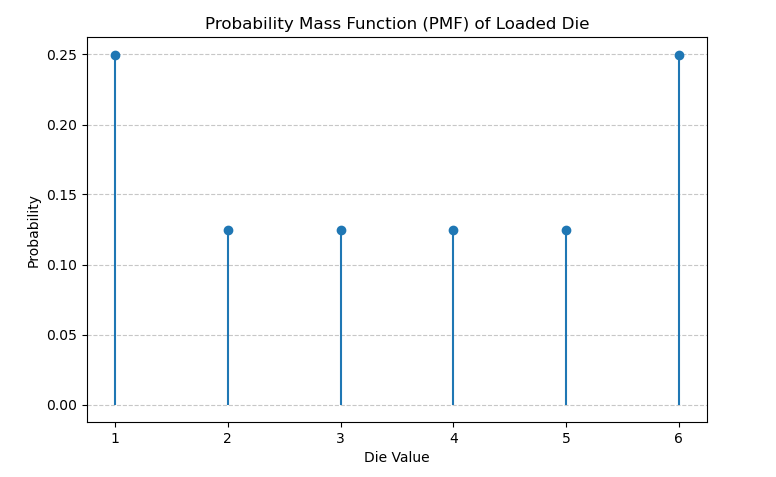
\includegraphics[width=0.9\columnwidth]{Figures/pmf.png}
\caption{PMF}
\label{fig:placeholder}
\end{figure}
\end{frame}

\begin{frame}{Numerically Calculated Probability}
The desired Probability is computed numerically by generating the distribution by rolling the dice 1000000 times.
\begin{figure}[H]
\centering
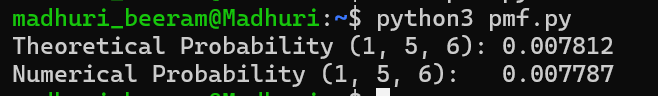
\includegraphics[width=1\columnwidth]{Figures/Numerical.png}
\caption{Output}
\label{fig:placeholder}
\end{figure}
Numerically found value closely matches with the calculated Probability.
\end{frame}
\end{document}